\documentclass{standalone}
\usepackage{tikz} 
\usetikzlibrary{arrows, decorations.markings,decorations.text,patterns,decorations.pathreplacing}
\usepackage{xcolor}
\usepackage{amsmath}
%\usepackage{BeamerColor}
\usepackage{microtype}
\usepackage{fourier}

\begin{document}

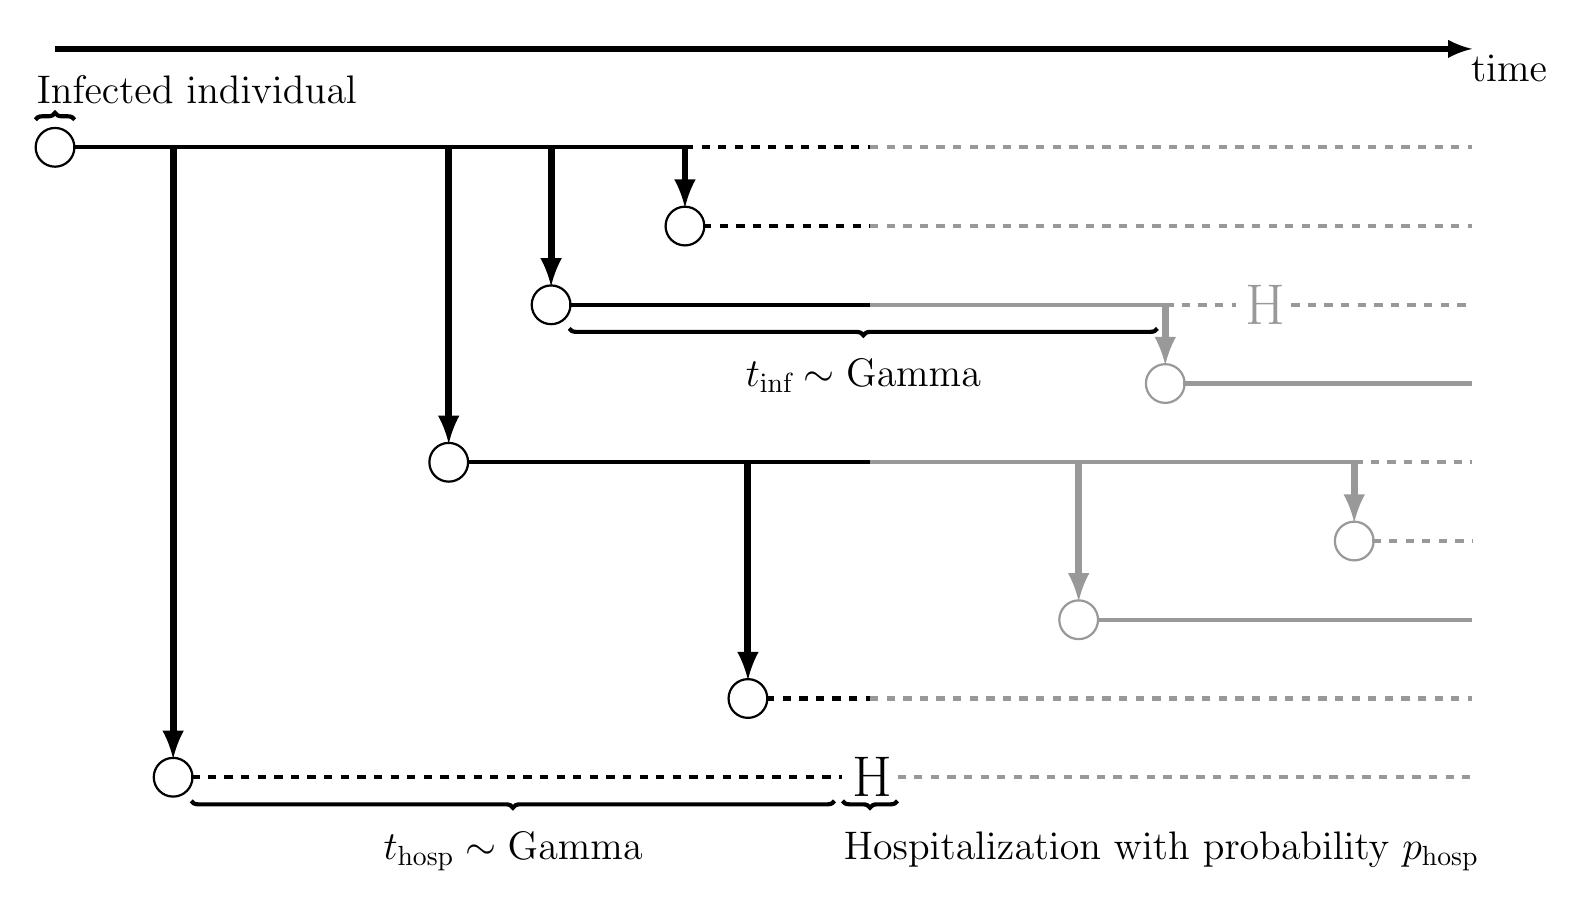
\begin{tikzpicture}
	
	% timeline
	\draw[-latex,line width=2pt,black] (0,0.25) -- (18,0.25) node [midway,above,sloped] {};
	\draw (18,0) node[right=-4pt] {\Large time};

   	% 1st individual	
	\draw[fill=white,thick] (0,-1) circle (7pt);
	\draw[line width=1.5pt] (0.23,-1) -- (8,-1);
	\draw[line width=1.5pt,dashed] (8,-1) -- (10.35,-1);
	\draw[line width=1.5pt,dashed,color=black!40] (10.35,-1) -- (18,-1);
	
	%2nd individual
	\draw[fill=white,thick] (1.5,-9) circle (7pt);
	\draw[-latex,line width=2.5pt] (1.5,-1) -- (1.5,-8.77);
	\draw[line width=1.5pt,dashed] (1.73,-9) -- (10,-9);
	\draw[line width=1.5pt,dashed,color=black!40] (10.7,-9) -- (18,-9);
	\node[right=0pt] at (10,-9) {\huge H};
	
	%3rd individual
	\draw[fill=white,thick] (5,-5) circle (7pt);
	\draw[-latex,line width=2.5pt] (5,-1) -- (5,-4.77);
	\draw[line width=1.5pt] (5.23,-5) -- (10.35,-5);
	\draw[line width=1.5pt,color=black!40] (10.35,-5) -- (16.5,-5);
	\draw[line width=1.5pt,color=black!40,dashed] (16.5,-5) -- (18,-5);
	
	%4th individual
	\draw[fill=white,thick] (6.3,-3) circle (7pt);
	\draw[-latex,line width=2.5pt] (6.3,-1) -- (6.3,-2.77);
	\draw[line width=1.5pt] (6.53,-3) -- (10.35,-3);
	\draw[line width=1.5pt,color=black!40] (10.35,-3) -- (14.1,-3);
	\draw[line width=1.5pt,color=black!40,dashed] (14.1,-3) -- (15,-3);
	\node[right=0pt,color=black!40] at (15,-3) {\huge H};
	\draw[line width=1.5pt,color=black!40,dashed] (15.7,-3) -- (18,-3);
	
	%5th individual
	\draw[fill=white,thick] (8,-2) circle (7pt);
	\draw[-latex,line width=2.5pt] (8,-1) -- (8,-1.77);
	\draw[line width=1.5pt,dashed] (8.23,-2) -- (10.35,-2);
	\draw[line width=1.5pt,dashed,color=black!40] (10.35,-2) -- (18,-2);
	
	%6th individual
	\draw[fill=white,thick] (8.8,-8) circle (7pt);
	\draw[-latex,line width=2.5pt] (8.8,-5) -- (8.8,-7.77);
	\draw[line width=1.5pt,dashed] (9.03,-8) -- (10.35,-8);
	\draw[line width=1.5pt,dashed,color=black!40] (10.35,-8) -- (18,-8);
	
	%7th individual
	\draw[thick,color=black!40,fill=white] (13,-7) circle (7pt);
	\draw[-latex,line width=2.5pt,color=black!40] (13,-5) -- (13,-6.77);
	\draw[line width=1.5pt,color=black!40] (13.23,-7) -- (18,-7);
	
	%8th individual
	\draw[thick,color=black!40,fill=white] (16.5,-6) circle (7pt);
	\draw[-latex,line width=2.5pt,color=black!40] (16.5,-5) -- (16.5,-5.77);
	\draw[line width=1.5pt,color=black!40,dashed] (16.73,-6) -- (18,-6);
	
	%9th individual
	\draw[thick,color=black!40,fill=white] (14.1,-4) circle (7pt);
	\draw[-latex,line width=2.5pt,color=black!40] (14.1,-3) -- (14.1,-3.77);
	\draw[line width=1.5pt,color=black!40] (14.33,-4) -- (18,-4);
	
	%labels
	\draw [line width=1.5pt, decoration = {brace,mirror,raise=0.3cm}, decorate] (6.53,-3) -- (14,-3) 
node [pos=0.5,anchor=north,yshift=-0.55cm] {\Large {$t_{\text{inf}} \sim \text{Gamma}$}}; 

	\draw [line width=1.5pt, decoration = {brace,mirror,raise=0.3cm}, decorate] (1.73,-9) -- (9.9,-9) 
node [pos=0.5,anchor=north,yshift=-0.55cm] {\Large {$t_{\text{hosp}} \sim \text{Gamma}$}}; 

	\draw [line width=1.5pt, decoration = {brace,mirror,raise=0.3cm}, decorate] (10,-9) -- (10.7,-9) 
node [pos=0.5,anchor=north,yshift=-0.55cm,xshift=3.7cm] {{\Large Hospitalization with probability $p_{\text{hosp}}$}}; 

	\draw [line width=1.5pt, decoration = {brace,raise=0.3cm}, decorate] (-.25,-0.95) -- (0.25,-.95) 
node [pos=0.5,anchor=north,yshift=1cm,xshift=1.8cm] {{\Large Infected individual}}; 
	
\end{tikzpicture}						

\end{document}